\documentclass[letterpaper,12pt]{article}
\usepackage[utf8]{inputenc}
\usepackage{fullpage}
\usepackage{courier}
\usepackage[margin=0.75in]{geometry}
\usepackage{listings}
\usepackage{color}
\usepackage{graphicx}
\usepackage[width=5in]{caption}
\usepackage{hyphenat}
\usepackage[section]{placeins}
\usepackage{cmll}
\usepackage{float}

% Format a sectionless paragraph
\newcommand*\unparagraph{
	\par
	\nopagebreak
	\vskip3.25ex plus1ex minus.2ex
	\noindent
}

% define extra colors
\definecolor{dkgreen}{rgb}{0,0.6,0}
\definecolor{purple}{RGB}{159,0,197}

% define the code listing format
\lstset{
	language=C++,
	basicstyle=\footnotesize\ttfamily,
	backgroundcolor=\color{white},
	showspaces=false,
	showstringspaces=false,
	frame=none,
	tabsize=3,
	keywordstyle=\color{purple},
	commentstyle=\color{dkgreen},
	stringstyle=\color{blue},
	escapeinside={\%*}{*)}
}

% define the title/header
\title{\Large CS 1428 Honors\\Lab 4}
\author{Jared Wallace}
\date{}

\begin{document}

\maketitle

\vspace{30mm}

\section*{Questions}

\begin{enumerate}
    \item (15 pts) The memory(RAM) for our processor has a very small capacity. It will only be 256
                   “cells” of storage, with each cell storing a single integer value. We will implement
                   the memory as an array. How can we declare this array of storage?
    \item (15 pts) As already mentioned in question 2, each instruction the user inputs will consist of
                   one, and only one, line. The format of each line is as follows:
    \begin{table}[H]
    \begin{center}
        \begin{tabular}{c|c|c|c}
            operation-code & data-cell-0 & data-cell-1 & data-cell-2
        \end{tabular}
    \end{center}
    \end{table}
                   The content placed in each data-cell depends on the instruction. For instance,
                   the arithmetic instructions will use data-cell-0 for the index of the memory(array)
                   cell to write \emph{to}, data-cell-1 as the index of the \emph{left} operand, and data-cell-2 as
                   the index of the \emph{right} operand. Accordingly, assuming we have a memory array that looks
                   like
    \begin{table}[H]
    \begin{center}
        \begin{tabular}{|c|c|c|c|c|c|}
            \hline
            value & 4 & 23 & 10 & 40 & 5\\ \hline
            index & 0 & 1 & 2 & 3 & 4 \\ \hline
        \end{tabular}
    \end{center}
    \end{table}
                   in order to subtract 23 from 10, and store the result in memory cell 0, we would
                   have the following line:

                   1(for subtract) 0(store in index 0) 1(index of 23) 2(index of 10)

                   Now write some code that reads in an instruction line, and then processes and performs
                   the appropriate instruction. (Remember, addition is 0, subtraction is 1,
                   multiplication is 2, division is 3, and exponentiation is 4)
                   (Hint: It would be much easier to use a switch statement, much like the “calculator”
                   we wrote last week)
    \item (15 pts) We also need to develop some read and write instructions to allow the program to
                   accept input from, and output to, the user. (Otherwise the assembler wouldn't be
                   very useful) Add the necessary lines to the switch statement you already have,
                   so that read and write instructions can be handled with the following format:
                   (the \emph{read} instruction accepts user input and stores it into the proper cell,
                   and the \emph{write} instruction takes the value of the specified cell and prints it
                   to standard out)
    \begin{table}[H]
    \begin{center}
        \begin{tabular}{c|c|c|c}
            5(op-code read) & index of the cell to store the value & 0 & 0 \\
            6(op-code write) & index of the cell to read from & 0 & 0 \\
        \end{tabular}
    \end{center}
    \end{table}
    \item (15 pts) Lastly, we need a way for the program to directly store constant values into its own
                   memory. This is done by the store command. If store is implemented as follows:
    \begin{table}[H]
    \begin{center}
        \begin{tabular}{c|c|c|c}
            7(op-code store) & index of the cell to store to & value to store & 0 \\
        \end{tabular}
    \end{center}
    \end{table}
                   add the additional lines necessary to your switch statement to implement the store
                   instruction.
    \item (40pts) Using the snippets you have written in the previous questions,
                  create a single program (lab4h.cpp) that:
                  \begin{itemize}
                      \item Prompts the user to enter the number of lines the program will have
                      \item Prompts the user line by line for the “code”
                      \item After the specified number of instruction lines have been entered,
                            the program should execute the inputted instruction lines.
                      \item You can test the correctness of your program by inputting the instruction
                          lines inside the supplied \emph{age.txt} file.
                  \end{itemize}

\end{enumerate}
\section*{Deliverables}
Hard copy of the source code you updated (assembler.cpp)
and the answers to the questions. Soft copy (upload to homework upload) of all your source code files.

\emph{Do not forget} to run the following commands to make a commit and "push" your changes!
\begin{lstlisting}
git add assembler.cpp
git commit -m 'Insert witty commit message here'
\end{lstlisting}

% Comic at the bottom
\begin{figure}[ht!]
	\centering
	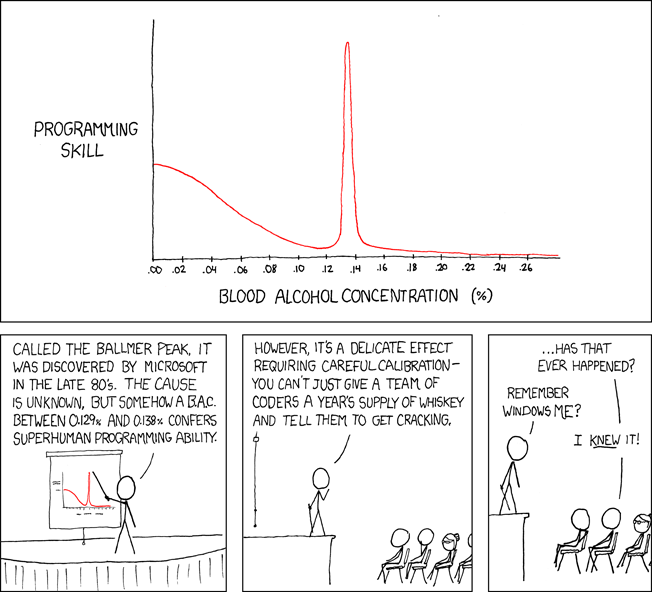
\includegraphics[width=5in]{ballmer_peak.png}
    \caption*{Apple uses automated schnapps IVs.}
\end{figure}
\end{document}
